\chapter{Edafología}
\begin{definition}[Suelo]
    Es un cuerpo natural y dinámico que posee propiedades y características del tipo físico, químico y biológico que forman un sistema
\end{definition}
En ésta definición, debemos considerar que un cuerpo, puede ser explicado como un ente que tiene materia y un lugar en el espacio, de manera que se puede cuantificar como:
\begin{equation}
    D = \frac{\text{Masa}}{\text{Volumen}}
\end{equation}

Si es natural, es porque el humano no ha modificado su uso, dinámico porque cambia a través del tiempo así como por el proceso de erosión eólica es transportada todo el tiempo.

\subsection{Proceso Pedogenéticos}

Son procesos que definen directamente las características y propiedades que diferenciarán los distintos suelos y se dan durante el desarrollo de este mismo. El tipo de procesos, así como la intensidad con la cual ellos actúan, es controlado por los factores de formación.

Los procesos pedogenéticos se pueden estudiar en varios niveles de detalle; por esta razón se clasifican en dos grupos fundamentales de procesos:

\begin{itemize}
    \item Globales
    \item Especificos o Particulares\begin{itemize}
        \item De adiciones
\item De transformaciones
\item De translocaciones
\item De pérdidas
\item Complejos
\item Andolización
\item Podzolización
\item Ferralitización
    \end{itemize}
\end{itemize}

El ``Littering'' es la acumulación de materiales orgánicos en la superficie del suelo, constituyendo el horizonte o epipedon hídtico; la ``Cumulización'' es la adición de partículas minerales a la superficie del suelo. Aporta a la acumulación de materia en los suelos aledaños a las áreas más desprotegidas.

\begin{definition}[Humificación]
    Transformación de los materiales orgánicos y frescos en humus.
Promueve la formación de los horizontes A.
\end{definition}

\begin{definition}[Mineralización]
    Transformación de cierto tipo de elementos formados por algunos compuestos orgánicos en varios compuestos inorgánicos.
Genera pérdidas netas de materia orgánica en él.
\end{definition}
\begin{definition}[Gleización]
    Compuestos ferrosos, Por condiciones reductoras en, el medio, Colores grises y manchas
\end{definition}
\begin{definition}[Rubefacción]
    Deshidratación progresiva de sesquióxidos de hierro, Enrojecimiento del suelo, En horizontes B cámbicos, Marronización y ferruginación
\end{definition}
\begin{definition}[Endurecimiento]
    Disminución de los poros por compactación, colapso de la estructura, rellenado de poros con otros materiales sólidos e Inundaciones
\end{definition}
\begin{definition}[Esponjamiento]
    Incremento en el espacio vacío por actividad de las plantas, los animales o del hombre
\end{definition}
\begin{definition}[Eluviación]
    Movimiento de materiales de salida de una porción del suelo; exportación de partículas desplazamiento por suspensión    
\end{definition}
\begin{definition}[Iluviación]
    Acumulación de materia, resultado del transporte desde un horizonte superior a uno inferior.
\end{definition}
\begin{definition}[Desalinización]
    Retiro de sales solubles en el agua del suelo.
\end{definition}
\begin{definition}[Decalcificación]
    Reacciones que retiran carbonato de calcio de algún horizonte del perfil de suelo
\end{definition}
\begin{definition}[Desalcalinización]
    Salida y acumulación de iones $Na^+$
\end{definition}
\begin{definition}[Lessivage]
    Migracion mecánica de pequeñas particulas de arcilla, dentro del solum.
\end{definition}

\begin{definition}[Edafoturbación]
    Mezcla que se hace de los materiales de alguna parte del solum; dependiendo del agente causal de la mezcla se establecen varios nombres para el proceso.
\end{definition}


\begin{definition}[Melanización]
    Es la acumulación de materiales orgánicos de color oscuro, en alguna porción del suelo, generalmente recubriendo sus partículas o sus agregados minerales y oscureciendo el horizonte en que se produce; en algunas ocasiones es un proceso de iluviación de humus.
\end{definition}

\begin{definition}[Leucinización]
Es la remoción de materiales orgánicos de color oscuro, puede ser un proceso de transformación de materiales orgánicos oscuros dentro del suelo.
\end{definition}

\begin{definition}[Desilicación]
Es la remoción de Si y es un proceso común en suelos de ambientes húmedos y con altas temperaturas.
\end{definition}

\subsubsection{Andolización}

Responsable de la formación de suelos Andisoles.
Se presenta una alteración no muy intensa de los materiales parentales cuyos productos forman nuevos materiales (síntesis) inorgánicos no cristalinos.
Se presenta una humificación importante de los residuos orgánicos que se adicionan al suelo; generalmente, hay lixiviación de bases.

\subsubsection{Podzolización}

Promueve la formación de suelos Espodosoles (mescla amorfa de materia orgánica, Al y Fe).
En el horizonte Espódico B se presentan procesos de rubefacción y marronización.
En el Horizonte eluvial E se presenta acumulación de sílice y leucinización.

\begin{definition}[Ferralitización]
    Proceso de Lixiviación intensa de bases y de sílice que genera acumulación de Fe. Es característico de climas tropicales.
    Llevan a la formación de suelos Oxisoles.
\end{definition}
\subsection{Formación de suelos}

Enfoque basado en los factores formadores
\begin{enumerate}
    \item Material parental, 
    \item clima
    \item geomorfología,
    \item vegetación y 
    \item tiempo.
\end{enumerate}

Metodología tipo ``caja negra'' (input y output). Si a la geomorfología se le da un papel especial: enfoque basado en las relaciones suelo-paisaje.

Enfoque basado en los procesos formadores

Metodología de ``caja gris'' y ``caja blanca''.

La clasificación de suelos, se basa en la función: Suelo= f(c,o,g,p,t)
\begin{figure}[h!]
\centering
  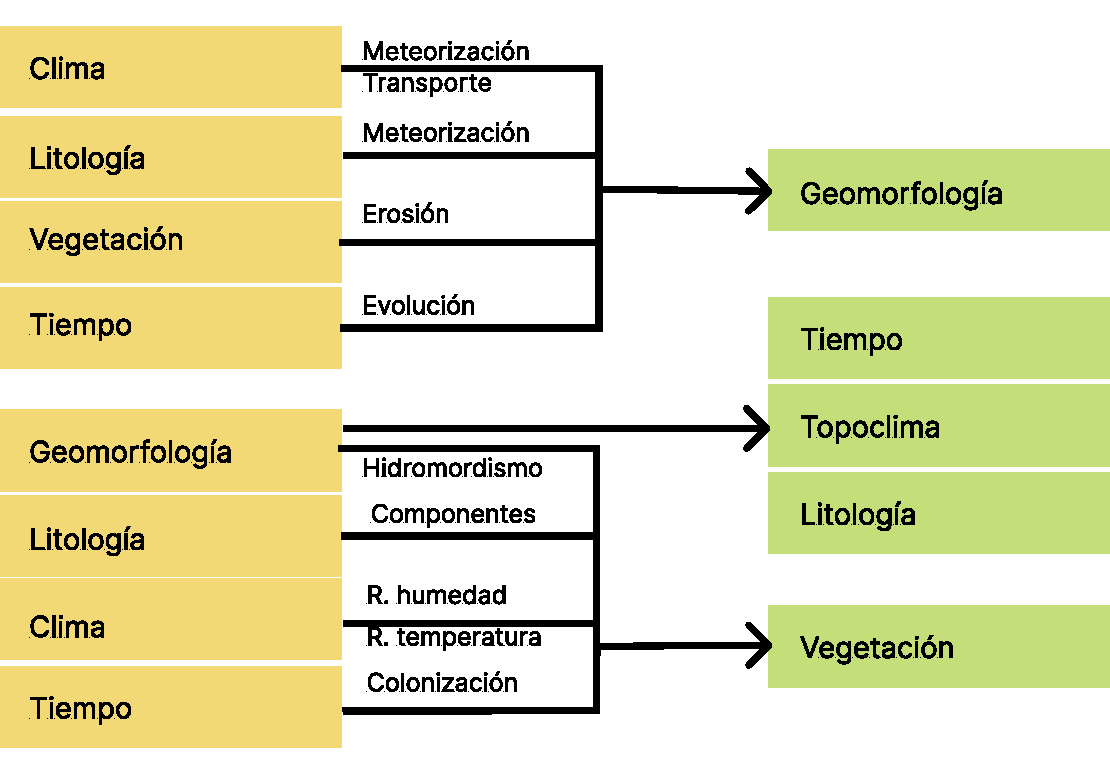
\includegraphics[width=0.5\textwidth]{ed5.pdf}
  \caption{Relación de las variables ambientales}
  \label{ed5}
\end{figure}
Con las iniciales de Clima, Organismos, (Factores activos); Topografía/relieve, Material parental y tiempo (Factores pasivos)

Los factores (Variables), no son independientes
La forma más simple de usar la relación es buscando suelos que estén relacionados por variación de uno sólo de los factores formadores:

\begin{align*}
    s=f(c)_{o,g,p,t}&&\text{Climosecuencia}\\
    s=f(o)_{c,g,p,t}&&\text{Biosecuencia}\\
    s=f(g)_{c,o,p,t}&&\text{Toposecuencia}\\
    s=f(p)_{c,o,g,t}&&\text{Litosecuencia}\\
    s=f(t)_{c,o,g,p}&&\text{Cronosecuencia}\\
\end{align*}

\begin{figure}[h!]
\centering
  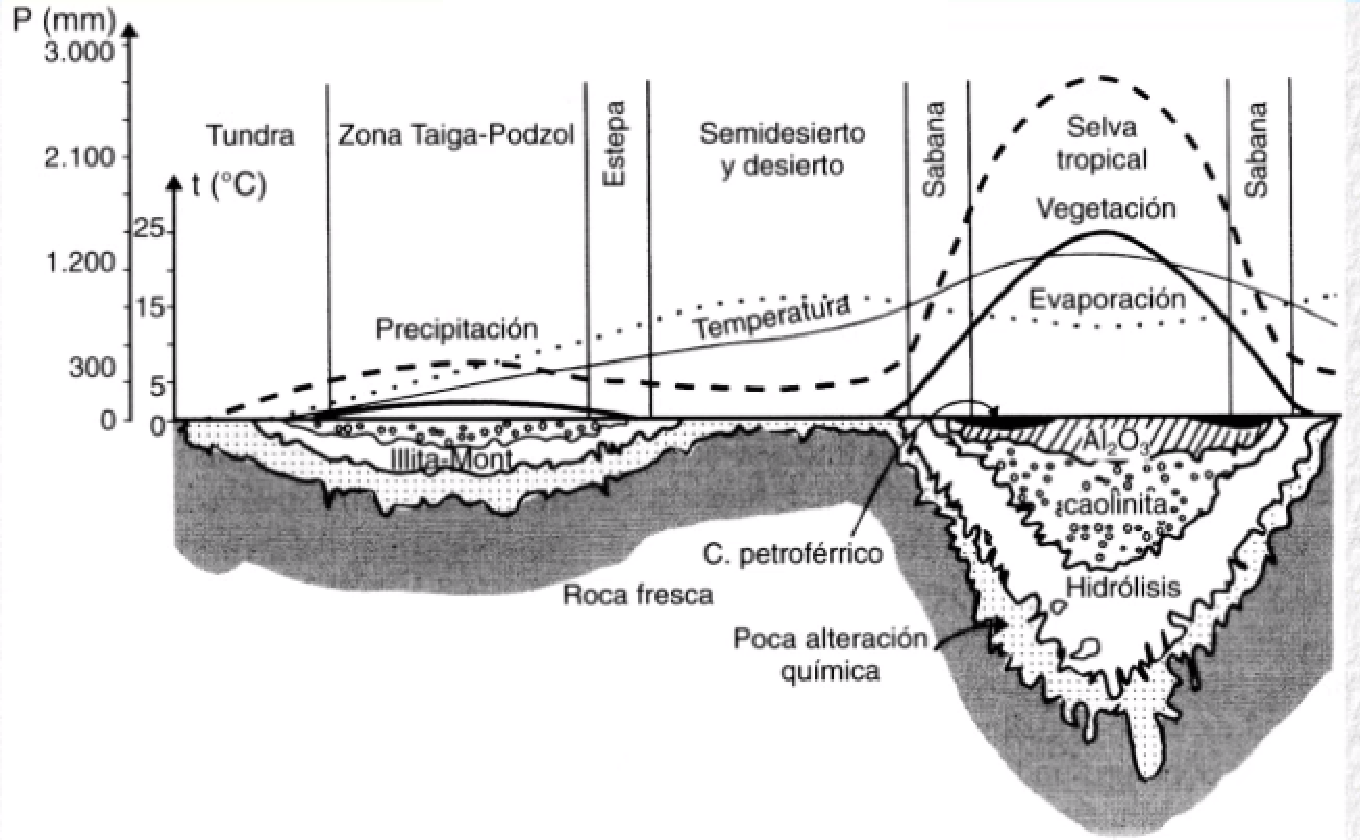
\includegraphics[width=0.5\textwidth]{ed4.pdf}
  \caption{Climoseciencias: Gelisol, inceptisol, Spodosol, Alfisol, Mollisol, Aridisol, Ultisol, Oxisol}
  \label{ed4}
\end{figure}

\begin{figure}[h!]
    \centering
    \begin{subfigure}[b]{0.45\linewidth}
    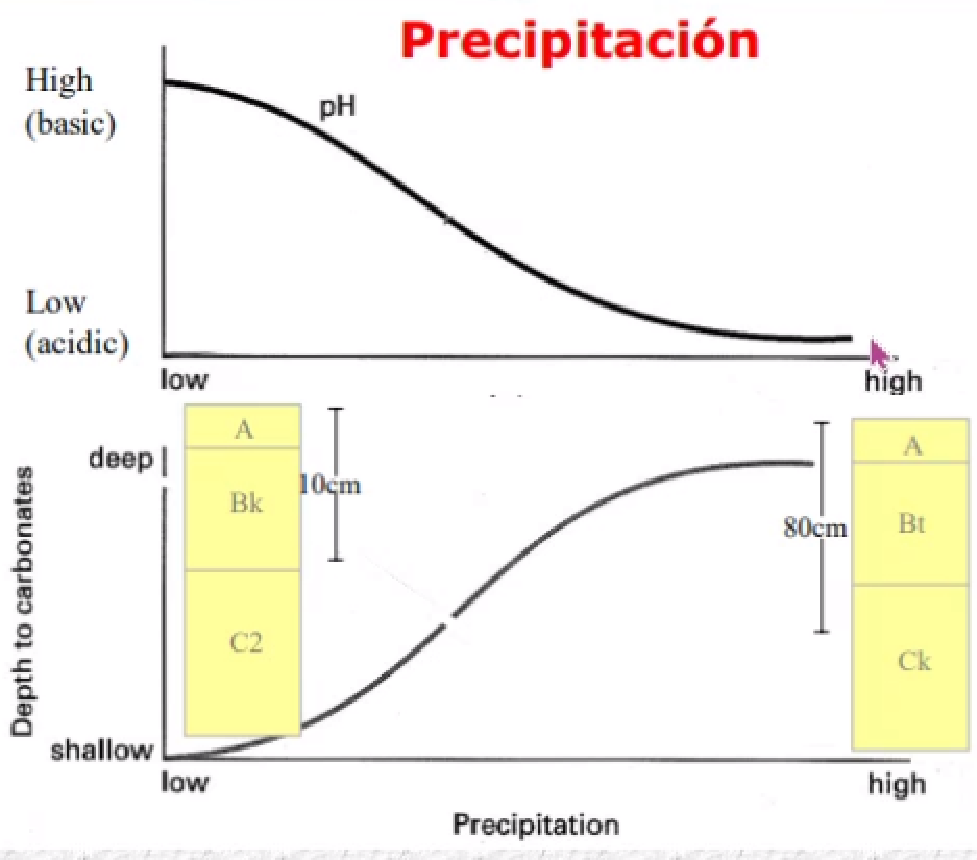
\includegraphics[width=\linewidth]{ed6.pdf}
    \caption{Precipitación}
    \label{ed6}
    \end{subfigure}
    \begin{subfigure}[b]{0.45\linewidth}
    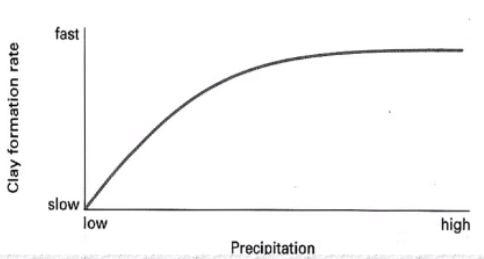
\includegraphics[width=\linewidth]{ed7.png}
    \caption{Proceso de lluvia}
    \label{ed7}
    \end{subfigure}
    \caption{Climatología}
    \label{ed6-7}
\end{figure}

\begin{figure}[h!]
\centering
  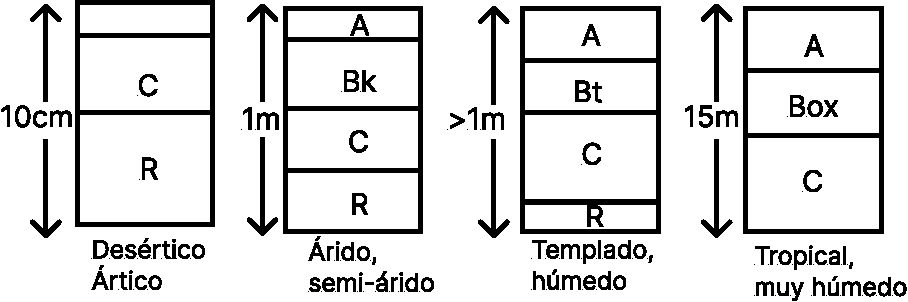
\includegraphics[width=0.5\textwidth]{ed8.pdf}
  \caption{Espesor del suelo y horizontes}
  \label{ed8}
\end{figure}
Los organismos como las plantas con sus raíces, composición de hojas; Microogranismos (Que descomponen la Materia Orgánica); Microfauna como lombrices, hormigas, topos crean huecos para el movimiento del agua, materia orgánica y estructura; Y seres humanos con la compactación cambios en el suelo; son aquellos que influyen la formación y características del suelo

Las especies indicadoras se hacen notables cuando hay:
\begin{itemize}
    \item acidez en el suelo (Toxicidad de Al)
    \item Plantas calcícolas y calcífugas
    \item Plantas halófitas
\end{itemize}
La vegetación favorece la meteorización; aporte de materia orgánica, y pantalla frente a la radiación solar y el viento.

\subsubsection{Geomorfología}

e\begin{definition}[Material parental]
    ES el material de partida, ``la condición inicial''. Los tipos de minerales tienen facilidad de meteorización, composición; abundancia relativa de cada mineral; tamaño de grano y materia orgánica
\end{definition}
\begin{figure}[h!]
\centering
  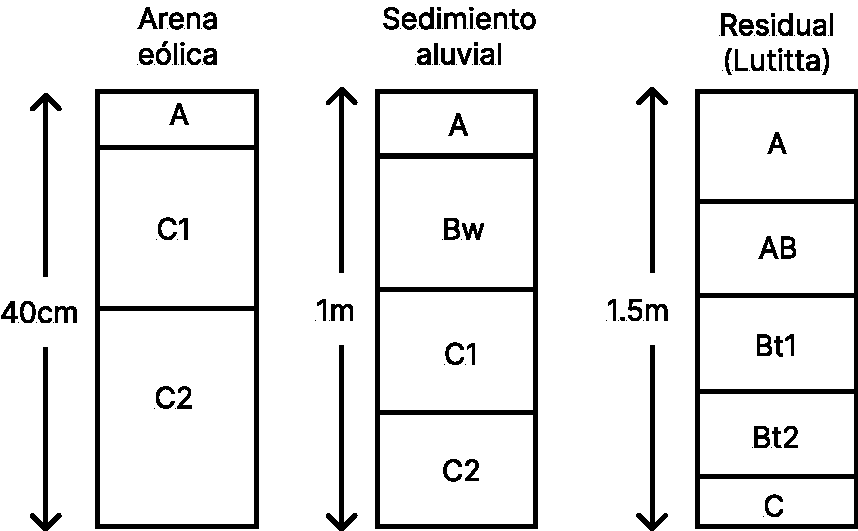
\includegraphics[width=0.5\textwidth]{ed9.pdf}
  \caption{Efecto del material prental sobre el suelo}
  \label{ed9}
\end{figure}

\subsection{Procesos formadores}
Según la teoría de Simonson (1959)m los procesos formadores del suelo se puede agrupar en cuatro categorías:
\begin{itemize}
    \item Adiciones al suelo (A)
    \item Pérdidas del suelo (P)
    \item Translocaciones dentro del suelo (Tl)
    \item Transformaciones dentro del suelo (TF)
\end{itemize}
Subdividir, informalmente en dos grupo:
\begin{itemize}
    \item \textbf{Proceso básicos}: 
    \begin{itemize}
        \item Transformaciones minerales (TF)
        \item Eluviación - iluviación (TL)
        \item Lixiviado (P)
        \item Edafortubación (TL)
        \item Acumulación de materia orgánica (A+TF)
    \end{itemize}
    \item \textbf{Procesos compuestos}: Resultan de la actuación simultánea o en cadena, de varios procesos básicos
\end{itemize}
Como adiciones:
\begin{itemize}
    \item Agua (superficial y subterránea)
    \item Material disuelto y en suspensión en el agua
    \item Sólidos transportados por el viento
    \item Gases de la atmósfera
    \item Energia del Sol
    \item Carbono orgánico de las plantas derivado de las raíces
    \item Carbono orgánico sintetizado por bacterias fotoautótrofas
    \item Nitrógeno orgánico sintetizado por bacterias fijadoras de N
    \item Restos de plantas y animales.
\end{itemize}
Pérdidas:
\begin{itemize}
    \item Material superficial por acción eólica
    \item Material eliminado por erosión
    \item Lixiviado de material disuelto (por la parte inferior)
    \item Absorción de nutrientes por las plantas
    \item $CO_2$ producido por plantas, animales y microbios
    \item Gases producidos por bacterias desnitrificantes
    \item Gases, como el metano, producidos por bacterias anaerobias.
\end{itemize}

Translocaciones por mezcla del material de diferentes horizontes (haploidización)
\begin{itemize}
    \item Animales (faunaturbación),
    \item Caída de árboles (floraturbación),
    \item Expansión y secado de suelos con arcillas,
    \item esmectíticas (argiloturbación),
    \item Hielo-deshielo (crioturbación),
    \item Terremotos (sismoturbación).
\end{itemize}

La \textbf{argiloturbación}, tienen griestas anchas y profundas (Slickensides) en el proceso principal en los \texttt{Vertisoles}.
Translocaciones conducentes a la formación de horizontes (horizonación):

Gradientes en el potencial hidráulico y en la concentración de solutos en los poros del suelo.
Se pueden mover verticalmente (hacia arriba y hacia abajo): minerales solubles, coloides, compuestos orgánicos en respuesta a movimientos del agua.
La actividad biológica también puede provocar gradientes de composición.

Los componentes del suelo son transformados por reacciones químicas.
Los compuestos orgánicos se descomponen, algunos minerales se disuelven, otros precipitan, otros se forman a partir de minerales primarios.
Estas transformaciones dan lugar a la estructura del suelo, cambios de color y la formación de horizontes.

\subsubsection{Calsificación}

Proceso por el cual se acumula carbonato cálcico en el perfil de un suelo.
Se produce en climas áridos y semiáridos, donde la evapotranspiración supera a la precipitación y el lixiviado es mínimo.
Los suelos afectados por calcifiación se agrupan en los Calcid (Aridisoles) y en los grandes grupos Calci- de Inceptisoles (e.g. Calcixerept), Mollisoles (e.g. Calcixeroll), Vertisoles (e.g. Calciustert).

La característica más obvia de estos suelos es la de poseer un horizonte cálcico (=Bk o Ck) o petrocálcico (-Bkm o Ckm) cuando la cementación es continua.


\begin{definition}[Gypsificación]
    Proceso por el cual se acumula yeso en el perfil de un suelo. Es un proceso menos general que la calcificación.
\end{definition}
\begin{definition}[Salinización y sodificación]
    Salinización: enriquecimiento superficial en sale más solubles que el yeso (sobre todo cloruros y sulfatos de sodio y magnesio) (TL).
    Proceso contrario: desalinización.
\end{definition}
\begin{definition}[Sodificación (=solonización)]
    Enriquecimiento en sodio intercambiable (TF). Suele ir acompañado de iluviación de arcillas, ya que el sodio favorece su dispersión. Proceso contrario: solodización.
\end{definition}
Los suelos en los que opera la salinización de forma natural son los antiguos Salonchak, ahora denominados \textbf{Salids} (con endopedión sálico Cz).
Los suelos en los que opera la sodificación ó solonización son los antiguos Solonetz, ahora incluidos en los grandes grupos que admiten el elemento formador Natr-(e.g. Natrargid, Natraqualf y Natraquoll), con endopedión nátrico (Btn).
\begin{definition}[Ferralitización]
Es la formación de un suelo por pérdida neta de sílice, formación de calinita y acumulación de óxidos, hidróxidos y oxi-hidróxidos de hierro y aluminio (principalmente hematites, goetita y gibsita).
Es un proceso exclusivo de regiones tropicales húmedas.
Da lugar a suelos potentes de tipo Oxisol.
\end{definition}
Los óxidos de Fe y Al iluviados forma un horizonte B óxico (Box). Para calificar como óxico, debe tener:
\begin{enumerate}
    \item al menos 30 cm de espesor,
    \item una textura franca arenosa o más fina,
    \item <10\% de minerales meteorizables,
    \item un límite sup. difuso, y    
    \item una CCC muy baja.
\end{enumerate}
\begin{definition}[Podzolización]
    Da lugar a suelos con buen desarrollo de horizontes y con predominio de vegetación acidificante (como el brezo o las coníferas). Este proceso no se da si hay carbonatos en el suelo.Son mayoritarios en las zonas frías y húmedas de la Tierra, como los bosques boreales de Canadá y Rusia (taiga).
Da lugar a los Spodosoles (entre otros).
\end{definition}
\subsection{Perfil edáfico y los horizontes}

El suelo es el material geológico no consolidado situado en la superficie de la tierra, generalmente a menos de 2m de profundidad.

\begin{definition}[Pedión]
    El volumen mínimo de material que s epuede reconocerse como un suelo individual y que oscila en tamaño entre 1 y 20 metros cúbicos
\end{definition}

\begin{definition}[Poliédión]
    Grupo de pediones similares contiguos que forman una unidad cartografiable. Los límites de un polipedión se alcanzan cuanod deja de haber suelo o cuando los pediones tienen unas características significativamente diferentes
\end{definition}

\begin{figure}[h!]
\centering
  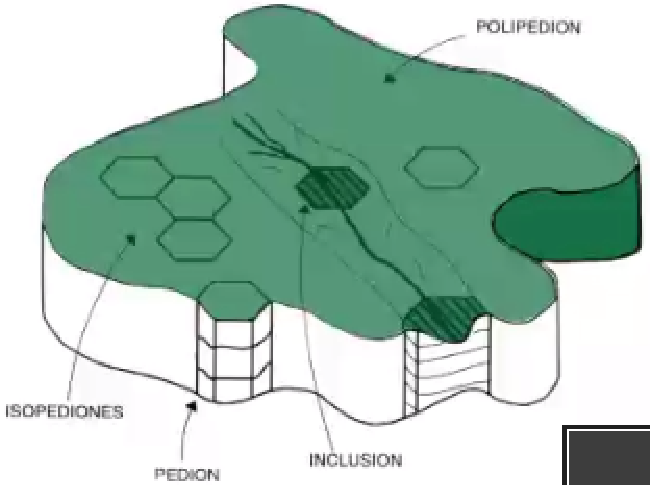
\includegraphics[width=0.5\textwidth]{ed10.pdf}
  \caption{El perfil edáfico}
  \label{ed10}
\end{figure}

\begin{definition}[Perfil edáfico]
    Sección vertical (2D) expuesta de los horizontes del suelo desec la superficie hasta el material infrayacente no edafizado.
\end{definition}
\begin{figure}[h!]
\centering
  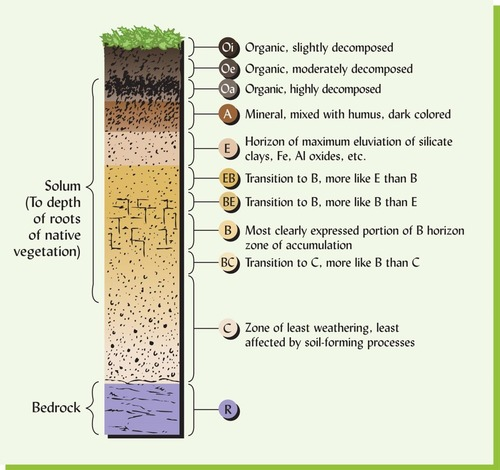
\includegraphics[width=0.5\textwidth]{ed11.jpg}
  \caption{Perfiles del suelo}
  \label{ed11}
\end{figure}

\begin{definition}[Horizonte edáfico]
    Es una capa horizontal aproximadamente paralela a la superficie, que difiere de las capas situadas, que difiere de las capas situadas por encima y por debajo en sus propiedades físicas, quiímicas o biológicas.
\end{definition}
Los horizontes de un suelo se nombran e identifican mediante una combinación de números, letras mayúsculas y letras minúsculas: (Número prefijo) Letra principal; (Letra sufijo) (Número sufijo)

\subsubsection{Horizonte O}
Horizonte orgánico formado, o en formación por acumulaciones de material orgánico, depositado sobrel la superficie, que no está saturado de agua más que unos pocos días al año y contiene 35\% o más de materia orgánica. La materia orgánica se encuentra poco o nada transfprmada, siendo claramente visible la organización biológica de los restos.

Por ejemplo la capa de hojarasca que recubre los suelos de bosque. Generalmente se les llama Histosoles a éste tipo perfil.

\subsubsection{Horizonte H}
Horizonte orgánico formado por acumulación de material orgánico depositado sobre la superficie, que está saturado de agua durante periodos prolongados, a menos que esté drenado artificialemnte y contiene 30\% o más de material orgánica, si la fracción mineral contienen más del 60\% de arcilla o 20\% o más de materia orgánica, si la fracción mineral no contiene arcilla o cantidades proporcionales intermedias de carbono orgánico para contenidos intermedios de arcilla.

Horizonte mineral formado, o en formación,
en la superficie que cumple una de las
siguientes condiciones:
\begin{enumerate}
    \item Presenta una acumulación de materia borgánica humificada, intimamente asociada con la fracción mineral, o.
    \item Tiene una morfología adquirida p\item formación del suelo, pero carece de l\item propiedades de los horizontes E y B
\end{enumerate}

\subsubsection{Horizonte E}

Horizonte mineral que presenta una elevada concentración de partículas gruesas (textura arenosa) como resultado de una pérdida de arcilla, hierro, aluminio, o alguna combinación de ellos.

Los horizontes E son horizontes eluviales que, generalmente están debajo de un horizonte A.

\subsubsection{Horizonte B}

Horizonte mineral en el cuál la estructura de
la roca está destruida o sólo queda
débilmente manifiesta, caracterizado por uno
o más de los rasgos siguientes:
\begin{enumerate}
    \item Una concentración iluvial de arcilla, hierro, aluminio o materia orgánica, solos o combinados;
    \item una concentración residual de sesquióxidos, con relación a los materiales de origen;
    \item una alteración del material, a partir de su condición original, tal que se forman arcillas, se liberan óxidos, o ambas cosas, o se produce una estructura granular, en bloques o prismática.
\end{enumerate}

\subsubsection{Horizonte C}
Horizonte mineral (o capa) de material no consolidado a partir del cual se supone que se ha formado un solum y que no presenta propiedades de diagnóstico de ningún otro horizonte principal.

Las acumulaciones de carbonatos, yeso u otras sales más solubles se pueden incluir dentro de los horizontes C si el horizonte está poco afectado por los procesos edáficos
\subsubsection{Horizonte R}
Capa de rocalcontinua endurecida. La roca de las capas R es suficientemente coherente, cuando está húmeda, para no permitir el cavar a mano con una azada. La roca puede presentar fisuras, pero éstas son demasiado escasas y demasiado pequeñas para permitir un desarrollo significativo de las raíces.

El material pedregoso que permite el desarrollo de raíces se considera también O como horizonte C.

\textbf{Las cifras prefijo}

Cuando es necesario distinguir discontinuidades litológicas, se usan cifras árabes como prefijos de la correspondiente denominación del horizonte.

Por ejemplo, cuando el horizonte C es diferente del material a partir del cual se supone que se ha formado el suelo, situado encima, se puede dar la siguiente secuencia: Ap, Bw, 2¢ Capas que contrastan fuertemente dentro del material C, se pueden presentar como una secuencia: Ap, E Bt, C, 2C, 3C,.

\subsubsection{Horizonte mezcla}
En algunas ocasiones aparecen horizontes principales mezclados. Están constituidos por zonas de un horizonte rodeadas por otras zonas correspondientes al otro horizonte.

Se designan con dos letras mayúsculas separadas por una raya inclinada (por ejemplo, E/B o B/C). La letra situada en primer lugar representa al horizonte más abundante.

\subsubsection{Letras sufifjo}

\begin{itemize}
    \item Cuando tiene el sufijo ``\textbf{b}'' de inglés burried, es un horizonte de suelo enterrado (Típico de fluvisoles) o bicíclico (p.e. Btb)
    \item Cuando tiene el sufijo ``\textbf{c}'' de concreción; Acumulación en forma de concreciones; este sufijo generalmente se usa combinado con otro que indica la naturaleza del material concrecionado (p.e Bck. Ccs)
    \item Cuando tiene el sufijo ``\textbf{g}'' del inglés gleying; Moteado (manchas rojas, amarillas y grises). Refleja variaciones en la oxidación y reducción como consecuencia de hidromorfia temporal (p.e.Bg, Btg, Cg).
    \item Cuando tiene el sufijo ``\textbf{h}'' Del lat. humus; Acumulación de materia orgánica en horizontes minerales (p.e. Ah, Bh); para el horizonte A. el sufijo h se aplica sólo en los casos de carencia de perturbación o mezcla por laboreo. pastoreo u otras actividades humanas (los sufijos h y p se excluyen mutuamente)
    \item Cuando tiene el sufijo ``\textbf{m}'' del inglés Massive; Fuertemente cementado, consolidado, endurecido; este sufijo generalmente se usa combinado con otro que indica el material cementante (p.e.Cmk para un horizonte petrocálcico, dentro de un horizonte C; Bms indica una costra de hierro, dentro de un horizonte B).
    %%%%%%%%%%%%%%%%%%%%%%%%%%
    \item Cuando tiene el sufijo ``\textbf{p}'' del inglés plouh; perturbación por laboreo u otra práctica agrícola
    \item Cuando tiene el sufijo ``\textbf{r}'' Reducción fuerte, como resultado de la influencia de la capa freática (p.e. Cr)m colores gris verdoso-azulados (Hidromorfía permanente)
    \item Cuando tiene el sufijo ``\textbf{s}'' De sesquióxidos; Acumulación de sesquióxidos de Fe y Al, generalmente de colores rijizos o amarillos
    \item Con el sufijo ``\textbf{t}'' del alemán ton; Acumulación de arcilla, casi siempre se trata de arcilla iluvial
    \item Con el sufijo ``\textbf{w}'' del inglés weathering; es la alteración in situ reflejada por el contenido de arcilla, el color o la estructura (p.e. Bw)
    \item Cuando el sufijo es ``\textbf{y}'' de yeso; tiene acumulación de yeso (p.e. Cy)
    \item Cuando el sufijo es ``\textbf{z}'' Acumulaciónes de sales más solubles que el yeso
\end{itemize}
\subsection{Intemperismo}
El intemperismo o meteorización es una parte básica del ciclo de las rocas y se produce por fragmentación física (desintegraicón), alteración química (descomposición) de las rocas de la superficie terrestre o por procesos biológicos. 
\subsubsection{Intemperismo físico}
Una roca experimenta intemperismo físico se rompe en fragementos cada vez más pequeños que conservan cada uno las características del material original:
\begin{itemize}
    \item Fragmentación por hielo
    \item Descomposición
    \item Expansión térmica
\end{itemize}
Los factores del intemperismo son:
\begin{itemize}
    \item Presencia de zonas (planos) de debilidad 
    \item Expansión provocada por la descompresión (Exfoliación esfenoidal y lajamiento)
    \item Fragmentación por hielo o gelificación: Se pueden observar fisuras
    \item Expansión y contracción térmica: En lugares con diferencias importantes de temperatura diurnas-nocturnas es un proceso que puede graduar este proceso
    \item 
\end{itemize}
\subsubsection{Intemperismo químico}
El intemperismo químico es el proceso mediante el cual los componentes de las rocas se descomponen por alteración química del material original. Es efectuado por la acción de los gases atmosféricos en especial el oxígen, el agua y los ácidos.
\begin{itemize}
    \item Hidrólisis
    \item Oxidación
    \item Disolución
    \item Carbonatación
    \item Reducción
\end{itemize}
\subsubsection{Intemperismo biológico}
El proceso de meterización biológica son una combinación de los efectos físicos y químicos. Se trata de un proceso de desgaste de la roca originado exclusivamente por seres vivos. Es común ver algunas raíces creciendo dentro de la cara de una roca.
\subsection{Productos de intemperismo}

La destrucción física y la alteración química de las rocas y minerales en la superficie de la tierra se conoce como intemperismo. Sus efectos o productos no se distribuyen de igual manera, debido a que las rocas no son uniformes.

\subsubsection{Bases}
Una base es cualquier sustancia que en disolución acuosa aporta iones $OH^{-}$ al medio. CUanto más básico sea el suelo más es el porcentaje de saturación de las bases. Cuanto más alto sea el porcentaje mayores posibilidades de retener cationes.
La saturación de bases es la suma de los cationes básicos $Ca^{2+}, Ng^{2+},K^{+},Na^{+}$.

\subsubsection{Arcillas}
De acuerdo a la clasificación de las fracciones granulométricas de los minerales del suelo de la USDA, las arcillas son partículas minerales menores a 0.002mm de diámetro. La arcilla es una fracción heterogénea constituida por minerales propios de la arcilla (aluminosilicatos, cristalino y amorfos), minerales no arcillosos o acompañantes (silicatos, óxidos, geles y otros).
Para comprender a las arcillas, estas son laminas de tetraedros como en la figura \ref{ed10png}
\begin{figure}[h!]
\centering
  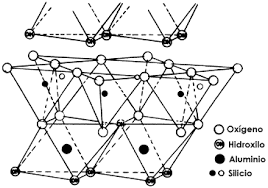
\includegraphics[width=0.5\textwidth]{ed10.png}
  \caption{Laminas de tetraedros y octaedros}
  \label{ed10png}
\end{figure}
Los elementos presentes son $Al,Mg,Fe^{3+}$.
Existen dos tipos de óxidos (ácido y básico), ambos son relativamente duros, densos y refractarios; se presentan de forma accesoria en rocas ígneas y metamórficas y como granos detríticos en los sedimientos, como ejemplo el dióxido de silicio
\begin{definition}[Dióxido de silicio]
    Los principales minerales silíceos como el cuarzo
\end{definition}
En el caso de las nases se sabe que en disolución acuosa producen iones negativos (aniones) OH sustituibles por residuos alogénicos o aniones ácidos para la formación de sales.

\begin{definition}[Arcillas]
    Son heredades del material originario sin apenas sufrir transformaciones; o ser el resultado de modificaciones, reorganización de los productos de meteorización y condiciones del suelo en general.
\end{definition}
En el caso de los óxidos, la liberación de aluminio, hierro, manganeso, titanio y silicio como resultado de los procesos de meteorización de minerales ferromagnesianos (biotitas, anfiboles y pirozenos) condice a la neoformación en el suelo.

\subsection{Composición de los suelos}
Los nutrientes deben de ser iónicas (déficit de electrónes), los signos representan la unión de dos átomos.
La caolinita y montmorillonita son dos minerales de la arcilla más importantes para la agricultua, el primero es una capa es de tetraedros y el segundo de octaedros.
La existencia de las caolinitas sirven para explicar los procesos metereológicos. La caolinita es 1:1 porque tiene una capa de tetraedros y una de octaedros mientras que la montmorillonita son tipo 2:1 son dos capas de tetraedros y una de octaedros, ésto son hilos envés de cíclos como otras arcillas.
Cristales amorfos o alofanos porque los cristales al ser medidos con rayos-x puesto que los rayos los traspasaba.
Presión temperatura y humedad son los factores que determinan la cristalización variada.
\begin{definition}[Sustitución Isomórfica]
    Cuando en las colas o extremos de los hilos de cristales, puede haber una sustitución de diferente estado de oxidación de un átomo
\end{definition}
\section{Análisis de suelo}

Se tiene un enfoque con el sistema Galvis (1998), anteriormente se maneja con fases (Sólida, Líquida y Gaseosa), pero
el autor esclareció que en realidad el sistema de análisis debe consistir en la fase sólida y \textbf{Porosa},
puesto que los líquidos y gases a través del suelo no puede analisarse, ahora el suelo no se verá como un cuerpo etereo, sino el suelo como sistema

Entiéndase un sistema como un conjunto de tiene un límite, componentes, Flujos, Entradas y salidas.

¿Cuáles serían los límites del suelo? desde el punto de vista edafológico la profundidad para la planta es lo relevante ya que hacia los laterales tenemos kilómetros de suelo.
Ahora la profundidad no está precismanete relacionada con la longitud de la raíz\footnote{Alometría es un término que se refiere al crecimiento exagerado de las raíces causado por el mejoramiento genético} porque existen diferentes tipos de raíces como:
\begin{itemize}
    \item Abasorción: Los pelos absorbentes están presente a 20cm a 30cm y por la presencia de oxígeno
    \item Anclaje: Se puede usar tutoraje para evitar el crecimiento desmedido de raíz
    \item Exploración: Indica estrés a mayor profundidad dependiendo del cultivo.
\end{itemize}
\begin{figure}[h!]
\centering
\begin{turn}{90}
  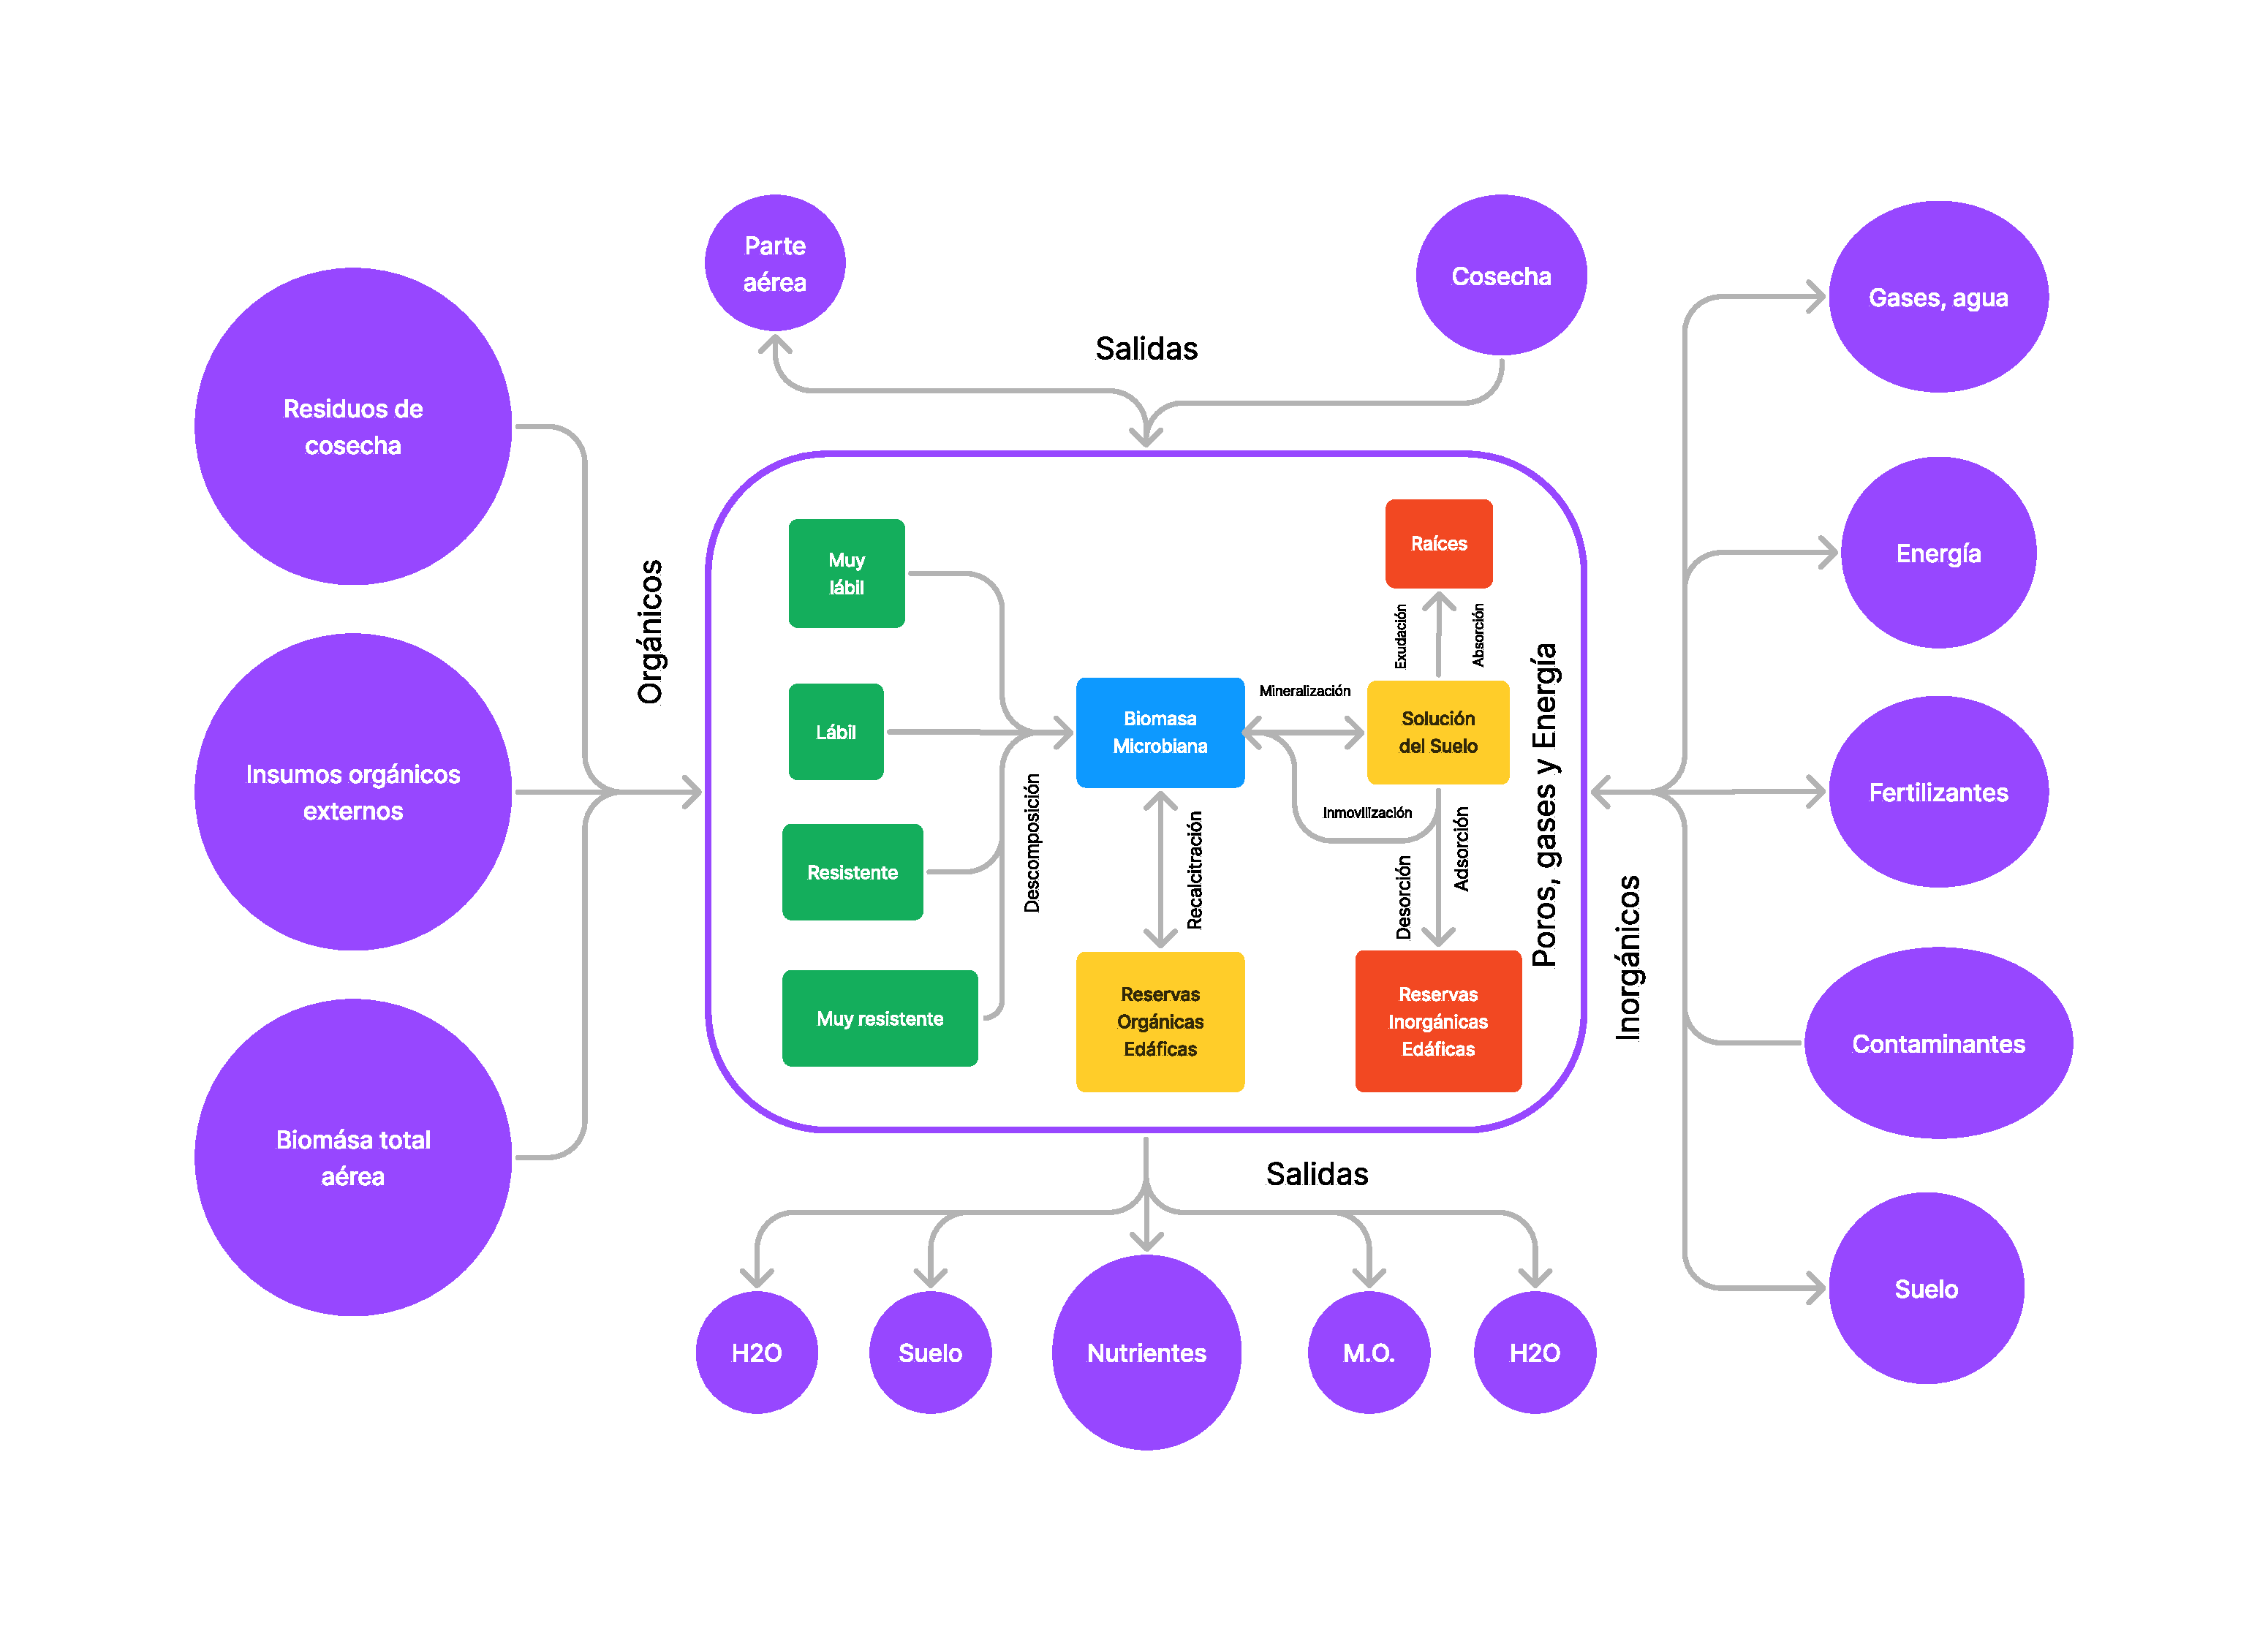
\includegraphics[width=1\textwidth]{ed12.pdf}
    \end{turn}
  \caption{Sistema del suelo}
  \label{ed12}
\end{figure}

% \subsection{Fertilidad}

\begin{definition}[Textura]
    Es la proporción de partículas primarias minerales e inorgánicas del tamaño arena, limo arcilla
\end{definition}

Se debe entender al suelo como una matriz, Es importante identidicar 
las clases texturales, el porcentaje debe ser manipulable, en el caso de las Arcillas
cuando las proporciones son 2:1 (Capacidad de absorción oscuras) 1:1 (Poca absorción de agua amarillos-rojos) las cuales están determinadas por el clima.

\section{Sistema del suelo}
Se identifican las propiedades físicas como:
\begin{itemize}
    \item Textura
    \item Color
    \item Densidad Real
\end{itemize}
Y en el caso de las características físicas:
\begin{itemize}
    \item Estructura
    \item Densidad Aparente
    \item Porosidad
    \item Infiltración
    \item Conducción Hidráulica
    \item Conductividad Térmica
\end{itemize}

Es importante destacar que las propiedades no se modifican mientras que las características del suelo sí lo hacen, por poner un ejemplo está la labranza cero y el barbecho: ambos tienen consecuencias en el suelo, en este caso la estructura es modificada para tener mejores rendimientos, pero en la labranza cero debido al ``mulch'' o restos del cultivo existía una compactación del suelo.

Protección de los materiales orgánicos: el agregado organo-mineral de tipo globular, tiene minerales y material orgánico. Tiene una estructura granular en la capa arable del suelo pues el mucilago (una sustancia de azúcares y sustancias orgánicas) interrumpe el intercambio de iones con las partículas del suelo y se forma ésta estructura.
Si se protegen los materiales revestidos con los materiales orgánicos. el tema es que al romper los agregados del suelo, la materia orgánica revestida del suelo se libera y se presenta la mineralización por parte de los microorganismos.

Si existe una densidad aparente mayor, habrá menor problemas de infiltración.
\begin{table}[h!]
    \begin{tabular}{@{}cccl@{}}
    \toprule
    Forma                                                                  & Tamaño    & Continuidad                                                             & Superficie            \\ \midrule
    Tortuoso                                                               & Macroporo & Continuos                                                               & Rugosa                \\
    \multirow{2}{*}{\begin{tabular}[c]{@{}c@{}}No\\ tortuoso\end{tabular}} & Mesoporo  & \multirow{2}{*}{\begin{tabular}[c]{@{}c@{}}No\\ continuos\end{tabular}} & \multirow{2}{*}{Lisa} \\
                                                                           & Microporo &                                                                         &                       \\ \bottomrule
    \end{tabular}
    \caption{Porosidad}
    \label{tabeda1}
\end{table}
Es deseable que el agua fluya en mesoporos para que la planta tenga el tiempo de absorberla, que sea continua (tortuosa),
pues pueden existir problema de inundación y la superficie se pretende ser rugosa porque hay más superficie específica (\textbf{Fertilidad física}).

Si son estables esos agregados en agua, entonces vuelven a reestructurarse, en caso contrario entonces no son organo-minerales.

\subsection{Saturación del suelo por Materiales Orgánicos}

\begin{definition}[Eutrofización]
    Es el aumento de nutrientes en los cuerpos de agua
\end{definition} 

Es un límite de la materia orgánica con respecto al tiempo.

\subsubsection{pH}
Es un indicador, una escala; la p es una función (Potencial) de hidrógeno. Es una convención que viene del agua pura, por ejemplo si tenemos un $K_p=\frac{\left[H^+\right]\left[OH\right]}{\left[H_2O\right]}$ lo que es equivalente a $1\times 10^{14}$, esto quiere decir que la concentración de hidrógeno $\left[H^+\right]=1\times 10^{-7}$ y la concentración de hidróxido $\left[OH\right]=1\times 10^{-7}$ por eso la escala es de 14 ($1\times 10^{-14}$).
Cuando se mide el pH en un suelo, indica la concentración del suelo, pH bajos se unen con Hierro, Cobalto, Manganeso, Zinc, Aluminio y pH altos con el Calcio, Magnesio, Potasio, Azufre y Sodio. 























